%% Creator: Inkscape inkscape 0.92.3, www.inkscape.org
%% PDF/EPS/PS + LaTeX output extension by Johan Engelen, 2010
%% Accompanies image file 'VortexCodeWorkFlow.pdf' (pdf, eps, ps)
%%
%% To include the image in your LaTeX document, write
%%   \input{<filename>.pdf_tex}
%%  instead of
%%   \includegraphics{<filename>.pdf}
%% To scale the image, write
%%   \def\svgwidth{<desired width>}
%%   \input{<filename>.pdf_tex}
%%  instead of
%%   \includegraphics[width=<desired width>]{<filename>.pdf}
%%
%% Images with a different path to the parent latex file can
%% be accessed with the `import' package (which may need to be
%% installed) using
%%   \usepackage{import}
%% in the preamble, and then including the image with
%%   \import{<path to file>}{<filename>.pdf_tex}
%% Alternatively, one can specify
%%   \graphicspath{{<path to file>/}}
%% 
%% For more information, please see info/svg-inkscape on CTAN:
%%   http://tug.ctan.org/tex-archive/info/svg-inkscape
%%
\begingroup%
  \makeatletter%
  \providecommand\color[2][]{%
    \errmessage{(Inkscape) Color is used for the text in Inkscape, but the package 'color.sty' is not loaded}%
    \renewcommand\color[2][]{}%
  }%
  \providecommand\transparent[1]{%
    \errmessage{(Inkscape) Transparency is used (non-zero) for the text in Inkscape, but the package 'transparent.sty' is not loaded}%
    \renewcommand\transparent[1]{}%
  }%
  \providecommand\rotatebox[2]{#2}%
  \newcommand*\fsize{\dimexpr\f@size pt\relax}%
  \newcommand*\lineheight[1]{\fontsize{\fsize}{#1\fsize}\selectfont}%
  \ifx\svgwidth\undefined%
    \setlength{\unitlength}{1584.33259703bp}%
    \ifx\svgscale\undefined%
      \relax%
    \else%
      \setlength{\unitlength}{\unitlength * \real{\svgscale}}%
    \fi%
  \else%
    \setlength{\unitlength}{\svgwidth}%
  \fi%
  \global\let\svgwidth\undefined%
  \global\let\svgscale\undefined%
  \makeatother%
  \begin{picture}(1,0.37987951)%
    \lineheight{1}%
    \setlength\tabcolsep{0pt}%
    \put(0,0){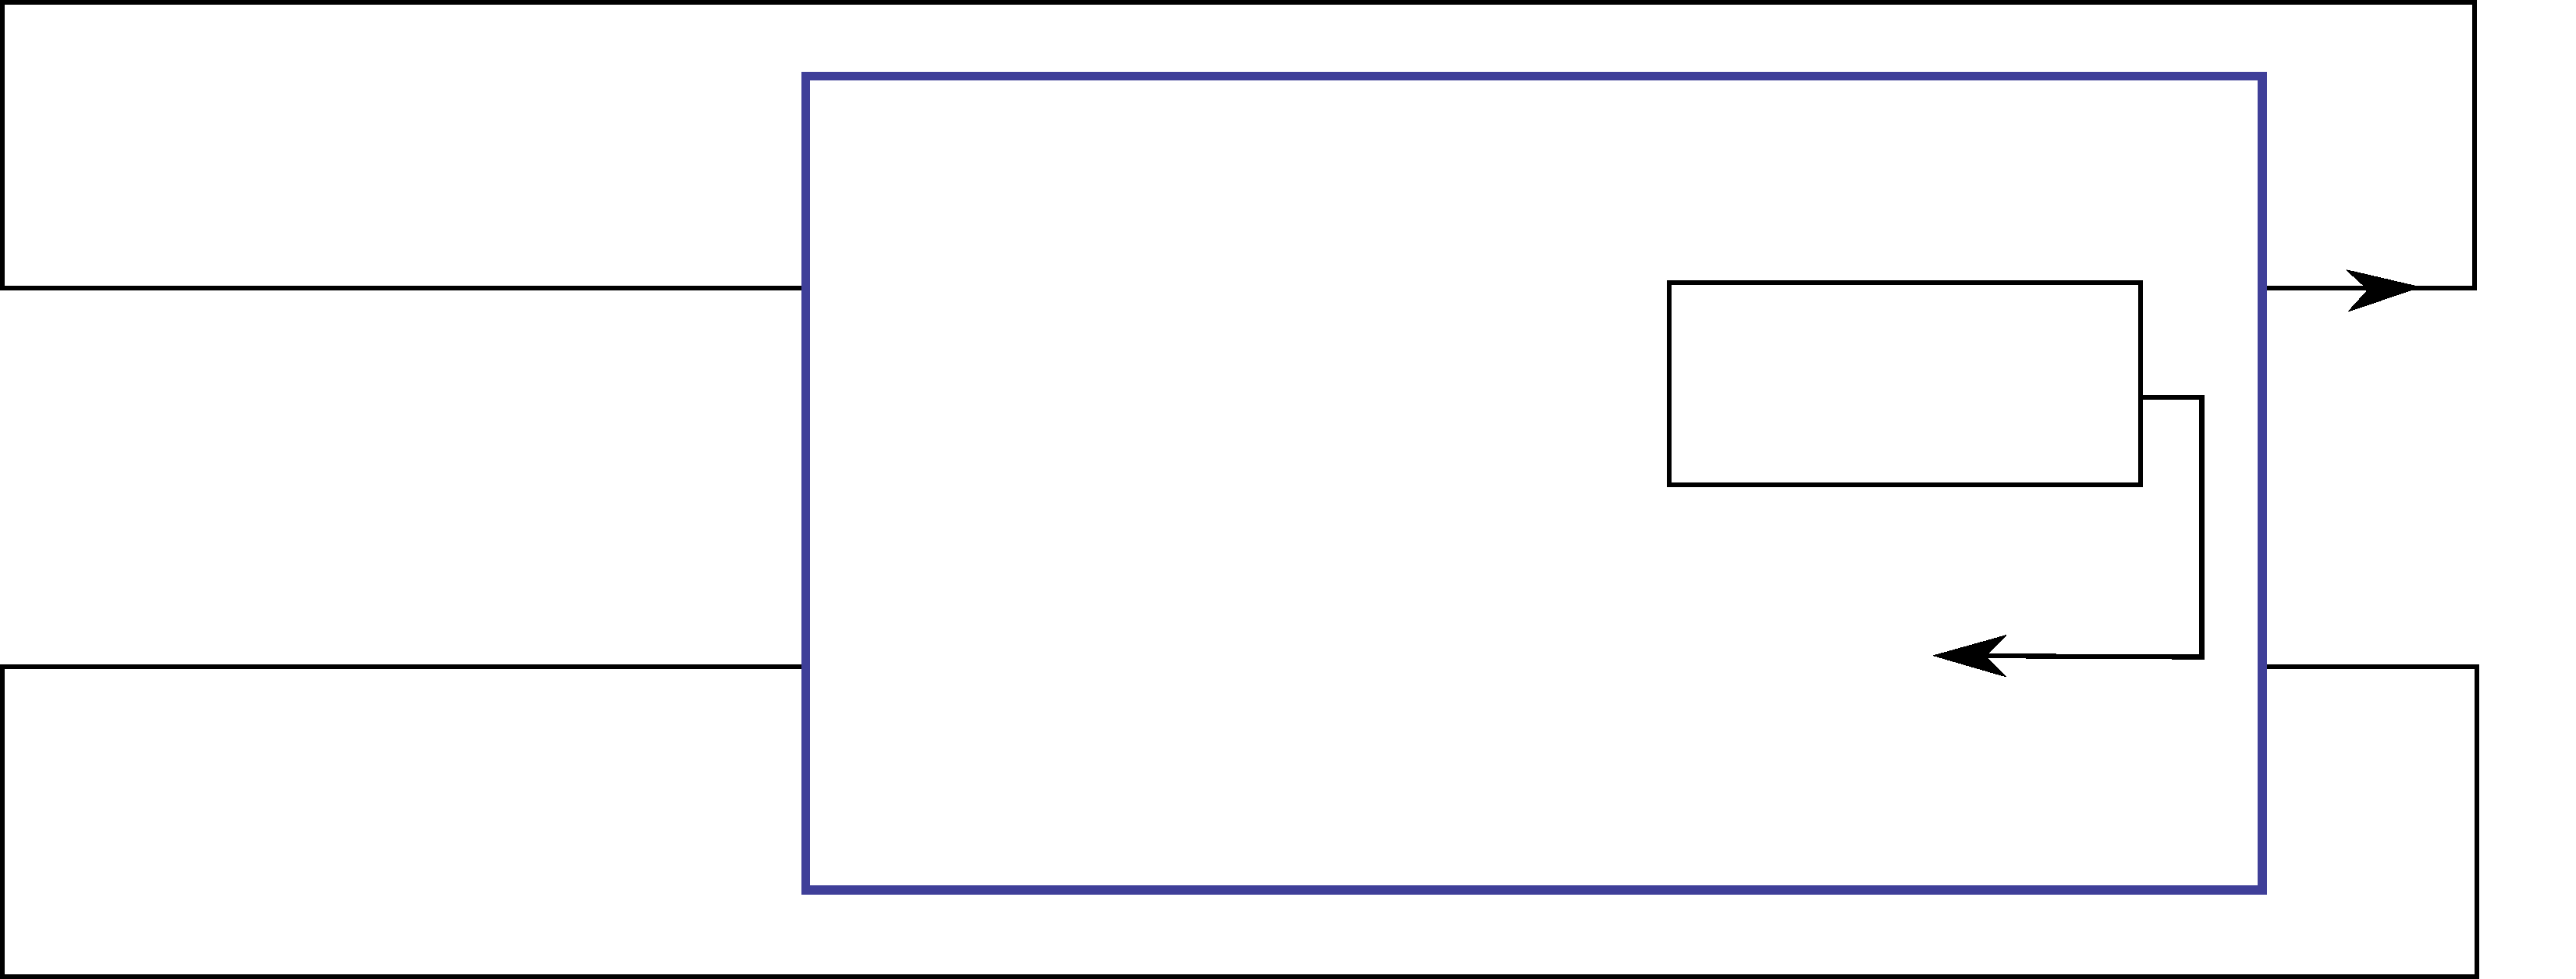
\includegraphics[width=\unitlength,page=1]{VortexCodeWorkFlow.pdf}}%
    \put(0.65944109,0.11446444){\color[rgb]{0,0,0}\makebox(0,0)[lt]{\begin{minipage}{0.25535428\unitlength}\centering $\vec{v}_{i,ll},  (\vec{r}_{r})$\end{minipage}}}%
    \put(0,0){\includegraphics[width=\unitlength,page=2]{VortexCodeWorkFlow.pdf}}%
    \put(0.63558708,0.20735708){\color[rgb]{0,0,0}\makebox(0,0)[lt]{\begin{minipage}{0.20717198\unitlength}\centering \textbf{Vortex code}\end{minipage}}}%
    \put(0.60215168,0.18502836){\color[rgb]{0,0,0}\makebox(0,0)[lt]{\begin{minipage}{0.27356877\unitlength}\centering $\vec{r}, \vec{\Gamma}_v$\end{minipage}}}%
    \put(0.32921211,0.30084711){\color[rgb]{0,0,0}\makebox(0,0)[lt]{\begin{minipage}{0.30485953\unitlength}\raggedright 1. Tower shadow model\\ \ \ \ \ (update of $\vec{V}_{\infty}$)\end{minipage}}}%
    \put(0.32826903,0.23341478){\color[rgb]{0,0,0}\makebox(0,0)[lt]{\begin{minipage}{0.3956149\unitlength}\raggedright 2. Induction computation\end{minipage}}}%
    \put(0.32826903,0.13392726){\color[rgb]{0,0,0}\makebox(0,0)[lt]{\begin{minipage}{0.5344643\unitlength}\raggedright 3. Quasi steady forces on the lifting lines\end{minipage}}}%
    \put(0.32826903,0.08442459){\color[rgb]{0,0,0}\makebox(0,0)[lt]{\begin{minipage}{0.51629305\unitlength}\raggedright 4. Dynamic stall model\end{minipage}}}%
    \put(0.49325791,0.33819968){\color[rgb]{0,0,0}\makebox(0,0)[lt]{\begin{minipage}{0.20355574\unitlength}\centering \textbf{AeroDyn15}\end{minipage}}}%
    \put(0.79169925,0.10320964){\color[rgb]{0,0,0}\makebox(0,0)[lt]{\begin{minipage}{0.25535428\unitlength}\centering $\vec{f}_{ll}$\end{minipage}}}%
    \put(0,0){\includegraphics[width=\unitlength,page=3]{VortexCodeWorkFlow.pdf}}%
    \put(0.79577993,0.29769798){\color[rgb]{0,0,0}\makebox(0,0)[lt]{\begin{minipage}{0.25535428\unitlength}\centering $\vec{r}_{ll}, \vec{r}_{r}$\end{minipage}}}%
    \put(0,0){\includegraphics[width=\unitlength,page=4]{VortexCodeWorkFlow.pdf}}%
    \put(-0.00885268,0.27822337){\color[rgb]{0,0,0}\makebox(0,0)[lt]{\begin{minipage}{0.20355574\unitlength}\centering \textbf{InflowWind}\end{minipage}}}%
    \put(0,0){\includegraphics[width=\unitlength,page=5]{VortexCodeWorkFlow.pdf}}%
    \put(0.69583824,0.27908716){\color[rgb]{0,0,0}\makebox(0,0)[lt]{\begin{minipage}{0.08495527\unitlength}\centering \textbf{BEM}\end{minipage}}}%
    \put(0,0){\includegraphics[width=\unitlength,page=6]{VortexCodeWorkFlow.pdf}}%
    \put(0.01537801,0.32400133){\color[rgb]{0,0,0}\makebox(0,0)[lt]{\begin{minipage}{0.44217675\unitlength}\centering $\vec{V}_\infty=$\\ $[\vec{V}_{\infty,ll}, \vec{V}_{\infty,r}] $\end{minipage}}}%
    \put(0.02471082,0.17907865){\color[rgb]{0,0,0}\makebox(0,0)[lt]{\begin{minipage}{0.41731078\unitlength}\centering $\vec{x}_{\text{elast},ll} =$\\ $ [\vec{r}_{ll}, \vec{\Lambda}_{ll}, \vec{\dot{r}}_{ll}, \vec{\omega}_{ll}]$\\ \end{minipage}}}%
    \put(0,0){\includegraphics[width=\unitlength,page=7]{VortexCodeWorkFlow.pdf}}%
    \put(-0.01097736,0.13673){\color[rgb]{0,0,0}\makebox(0,0)[lt]{\begin{minipage}{0.20355574\unitlength}\centering \textbf{ElastoDyn}\end{minipage}}}%
    \put(0.57551823,0.27600282){\color[rgb]{0,0,0}\makebox(0,0)[lt]{\begin{minipage}{0.41731078\unitlength}\raggedright $\vec{r}_{\text{elast},ll}$\\ $\vec{V}_\infty$\end{minipage}}}%
  \end{picture}%
\endgroup%
